\documentclass[a4paper,11pt]{article}
\usepackage{multicol}
%\usepackage{multitoc}
%\usepackage{german}
%\usepackage{bibgerm}
\usepackage{amsmath}
\usepackage{amsfonts}
\usepackage{xspace}
\usepackage[body={148mm,240mm,nohead}]{geometry}
\usepackage[ansinew]{inputenc}
\usepackage{listings}
\usepackage{tikz}
\usepackage{hyperref}
\lstset{language=C++, basicstyle=\ttfamily,
  stringstyle=\ttfamily, commentstyle=\it, extendedchars=true}

\newcommand{\dune}{\textsc{Dune}\xspace}
\newcommand{\modulename}[1]{\texttt{#1}\xspace}

\title{The dune-localfunctions module}

\author{The \dune Team}

\date{\today}

\begin{document}

\maketitle

\begin{abstract}
This document describes the \modulename{dune-localfunctions} module.
The module provides a C++ interface for shape functions needed in
finite element methods.  A growing list of implementations of this
interface is included. \modulename{dune-localfunctions}
is part of the Distributed and Unified Numerics Environment (\dune) which is
available from the site \url{http://www.dune-project.org/}.
\end{abstract}

\begin{multicols}{2}
{\small\tableofcontents}
\end{multicols}

\section{Introduction}

A feature common to all implementations of finite element methods are the
shape functions.  In the easier cases, these are polynomial functions
defined on a reference element and associated to some face of the reference
element.  The more complicated non-affine finite elements generalize this
by defining the shape functions directly on an element in the grid.

Implementations of shape functions are contained in all finite element codes,
but in most cases their implementation is so intertwined with the rest of
the code as to make their reuse in other situations impossible.
For the easier shape functions this may not matter much, as they are
fairly easy to implement.  Still, errors can occur and bugs in shape function
implementations can be difficult to detect and track down.
More exotic shape function implementations can get fairly involved
and require meticulous care to be done right.  For these reasons it is
very desirable to provide shape functions in a separate, reusable library.
This is what the \modulename{dune-localfunctions} module tries to do.


Following the UNIX philosophy of having each program doing only one thing,
but doing that thing well, the \modulename{dune-localfunctions} module
provides only local and global finite elements.  There are two sides to this.
\begin{enumerate}
 \item \modulename{dune-localfunction} prescribes an {\em interface} to shape functions.
  This interface
  should be general enough to encompass the needs of virtually all implementors
  of finite element codes.
 \item The module contains {\em implementations} of this interface.  The set
  of implementations contains common elements like the Lagrange elements and
  exotic ones as well.  We aim to collect contributions from outside sources
  and, in time, to be able to provide a shape function library that is virtually
  complete.
\end{enumerate}

\subsection{Static vs.\ Dynamic Interfaces}

From a textbook C++ perspective, an interface to finite element shape functions
can be described naturally using dynamical polymorphism.  An abstract base
class would describe all methods expected from a shape function implementation,
and actual implementations would derive from the base class.  Users of shape functions,
such as finite element assemblers, would receive shape function implementations
through pointers to the abstract base class.

However, the run-time overhead of virtual function calls is considered prohibitive
by some users.  We measured a slowdown of around 7\% when assembling a Laplace
stiffness matrix on a two-dimensional structured grid.  This can be relevant,
for example, in an explicit time-stepping method where a large percentage of
the overall time is spent assembling matrices.

We have therefore opted for a different way.  In \modulename{dune-localfunctions},
the implementation classes are {\em not} organized in a hierarchy.  Adherence
to a certain interface is enforced only implicitly, by a test suite.  Finite
element assemblers have to have the C++ type of the shape function implementation
as a template parameter, and can then call the object's methods directly.
The static interface is described in Section~\ref{sec:static_interface}.

Of course such a scheme makes it impossible to select shape function sets at run-time.
For example, $p$-adaptive methods, and methods on grids with more than a single
element type are precluded.  Therefore, \modulename{dune-localfunctions} offers
a second way to access its shape functions.  There is a set of {\em wrapper classes},
which are organized in a hierarchy using dynamical polymorphism.  These
wrapper classes are statically parametrized with a static implementation class
and forward the function calls to this implementation.  Details of this
{\em dynamic interface} are given in Section~\ref{sec:dynamic_interface}.

\subsection{Dependencies on other Modules}

When designing the \modulename{dune-localfunctions} module we have deliberately
tried to keep dependencies on other \dune modules to a minimum.  Ideally,
people should be able to use the shape functions from \dune without having
to use anything else from \dune.  The only exception here is \modulename{dune-common},
which all \dune modules depend on.

In addition to \modulename{dune-common}, \modulename{dune-localfunctions} currently
depends only on \modulename{dune-grid}.  This dependence is somewhat unfortunate,
and it has been hotly debated.  We would like users to be able to use \dune grids
without shapefunctions from \modulename{dune-localfunctions} and the shapefunctions
from \modulename{dune-localfunctions} without the grids from \modulename{dune-grid}.
While the former is easy, \modulename{dune-localfunctions} currently needs a few
features from \modulename{dune-grid} to work.  These are in particular a few
quadrature rules and some of the infrastructure for constructing reference elements.
More seriously, \modulename{dune-localfunctions} provides some {\em global} finite
elements (also known as {\em non-affine families} of finite elements).  These
have to have some information about the geometry of the grid.

In the future the necessary things from \modulename{dune-grid} may be split off
into a separate module \modulename{dune-geometry} (or similar).  The dependence of
\modulename{dune-localfunctions} on \modulename{dune-grid} can then be replaced
by the weaker dependency on the new module.


\section{The LocalFiniteElement Interface}
\label{sec:static_interface}

\subsection{The LocalBasis Classes}

\subsection{The LocalCoefficients Classes}

\subsection{The LocalInterpolation Classes}


\section{The Dynamic Interface}
\label{sec:dynamic_interface}

\section{Global Finite Elements}

So far this document has talked about finite elements on reference elements.
However, the finite element is usually needed on an element of a grid.  To
evaluate a function represented by a finite element basis on a particular grid
element $T$ with geometry $\mu$ we can use the following formula:
\begin{equation}
  u(x)=\sum_{i=0}^{N_T-1}c_iP_{T,i}\varphi_i(\mu^{-1}(x)) \qquad\forall x\in T
\end{equation}
The basis function $\varphi$ on the reference element is provided by the local
basis which was described previously.  The global basis takes this local basis
and applies an operator $P_{T,i}$ to the values it returns.  This operator is
dependent on the grid element $T$ and the number of the basis function $i$.
The global basis thus provides values of the global basis functions
\begin{equation}
  \Phi_i(\hat x)=P_{T,i}\varphi_i(\hat x)
\end{equation}

For the transformation $P$ the following information about grid element is
important:
\begin{enumerate}
\item The {\em geometry} $\mu$ of a grid element, which handles the
  transformation of coordinates from the reference element to the grid
  element.  But {\em values} of the base functions and in particular their
  derivatives need to be transformed as well in general -- the correct
  transformation depends on the family of the finite element, the coordinate
  transformation $\mu$ and the number of the base function $i$.
\item The {\em topology} $\tau$ of a grid element, which says how the grid
  elements vertices a globally numbered in comparison to the numbering in the
  reference element.  This is needed for vector valued finite elements such as
  Raviar-Thomas and edge-elements.  Here the dofs often have an orientation
  which can be chosen arbitrary but must match for all shape function of the
  same dof (but from different grid elements).
\end{enumerate}

This section explicitly does not deal with the following issues:
\begin{itemize}
\item Different geometry types for different grid elements.  This will lead to
  different number of basis functions and must already be dealt with in the
  local finite element.
\item $p$-adaptiviy.  Again, this will lead to different number of basis
  functions and must already be dealt with in the local finite element.
\item Renumbering of base functions.  This may be required for things like Q3
  which have multiple dofs on a given face and assign specific positions
  inside the face to those dofs.
\end{itemize}


\subsection{Topology}

The topology information is based completely on the global numbering of the
vertices of a grid element.  To obtain it, we collect the global IDs of the
vertices in a vector indexed by the indices of the vertices within the
reference element:
\begin{lstlisting}
void collectVertexIds(const Element& e, const GlobalIdSet& idSet,
                      std::vector<GlobaIdSet::IdType>& ids) {
  ids.resize(e.geometry().corners());
  for(int i = 0; i < ids.size(); ++ids)
    ids[i] = idSet.subId(e, i, Element::dimension);
}
\end{lstlisting}
In the next step the {\em topological reduction} operation is applied: the
smallest id in the array is replaced by the number 0, the second-smallest is
replaced by the number 1 etc.
\begin{lstlisting}
template<class LessThanComparable>
void topologicalReduction(const std::vector<LessThanComparable>& ids,
                          std::vector<std::size_t>& reduced) {
  std::vector<std::pair<LessThanComparable,std::size_t> > list(ids.size());
  for(std::size_t i = 0; i < ids.size(); ++i)
    list[i] = std::make_pair(ids[i], i);
  std::cout << list << std::endl;
  std::sort(list.begin(), list.end());
  std::cout << list << std::endl;
  reduced.resize(list.size());
  for(std::size_t i = 0; i <= list.size(); ++i)
    reduced[list[i].second] = i;
}
\end{lstlisting}
As an example, lets assume we have a quadrilateral or a tetrahedron with the
global ids of the vertices being 14 for vertex 0, 27 for vertex 1, 3 for
vertex 2 and 800 for vertex 3.  After topological reduction the reduced vector
will contain 1, 2, 0 and 3 in that order.

To ensure continuity for vector finite elements, we need to assign an
orientation to sub-entities shared by neighbouring grid elements.  Ideally,
this will work even if both neighbouring grid elements are of different
geometry type.

There is a distinction between local and global orientation: the local
orientation is the orientation according to the indices of the sub-entity's
vertices in the reference element.  The global orientation is the orientation
according to the global ids of the sub-entity's vertices within the grid.  If
the two orientations differ for a given grid element, the basis functions for
dofs on that sub-entity must be multiplied by $-1$.

\subsubsection{Line Orientation in 2D}

In 2D, the interface between two neighbouring elements is always a line.  For
lines in 2D there are however two different meanings of the term orientation,
depending on the finite element family.  Edge elements orient their dof along
the line, while Raviar-Thomas elements orient their dof perpendicular to the
line.  These two meaning are however compatible: the perpendicular orientation
can be obtained by turning the parallel orientation by $\pi/2$.  The rotation
must be perpendicular to the 2D-plane and should not flip -- this can be
achieved even for 2D manifold in a 3D space, unless you use something like a
M�bius strip.

The orientation of lines in 2D is from the lower index/id to the higher
index/id.

\subsubsection{Line Orientation in 3D}

In 3D the double-meaning of orientation does not occur.  This is not out of
principle, but just because I can only come up one family of finite elements
requiring orientation: edge elements.  The orientation of lines in 3D is
determined in the same way as for 2D: it is from the lower index/id to the
higher index/id.

\subsubsection{Triangle Orientation in 3D}

For 2D-entities in a 3D space we choose a face normal vector as the meaning of
the orientation.  If you look at a triangle and the reduced indices/ids of the
vertices run clockwise, the orientation vector points away from you, otherwise
it points towards you:

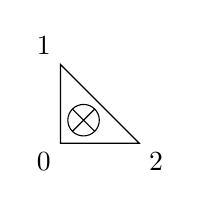
\begin{tikzpicture}
  \draw (0,0) node[below left] {0}
     -- (1,0) node[below right] {2}
     -- (0,1) node[above left] {1}
     --cycle;
  \coordinate (c) at (.29289,.29289);
  \draw (c) circle (.2);
  \draw (c) +(45:.2) -- +(45:-.2)
            +(-45:.2) -- +(-45:-.2);
\end{tikzpicture}
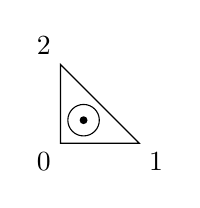
\begin{tikzpicture}
  \draw (0,0) node[below left] {0}
     -- (1,0) node[below right] {1}
     -- (0,1) node[above left] {2}
     --cycle;
  \coordinate (c) at (.29289,.29289);
  \draw (c) circle (.2);
  \fill (c) circle (.05);
\end{tikzpicture}

\subsubsection{Quadrilateral Orientation in 3D}

For quadrilaterals the numbering can be cyclic or acylic.  For the cyclic case
we choose the same rule as for the triangles: If you look at a triangle and
the reduced indices/ids of the vertices run clockwise, the orientation vector
points away from you, otherwise it points towards you.

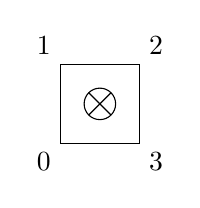
\begin{tikzpicture}
  \draw (0,0) node[below left] {0}
     -- (1,0) node[below right] {3}
     -- (1,1) node[above right] {2}
     -- (0,1) node[above left] {1}
     --cycle;
  \coordinate (c) at (.5,.5);
  \draw (c) circle (.2);
  \draw (c) +(45:.2) -- +(45:-.2)
            +(-45:.2) -- +(-45:-.2);
\end{tikzpicture}
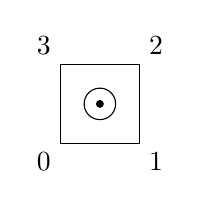
\begin{tikzpicture}
  \draw (0,0) node[below left] {0}
     -- (1,0) node[below right] {1}
     -- (1,1) node[above right] {2}
     -- (0,1) node[above left] {3}
     --cycle;
  \coordinate (c) at (.5,.5);
  \draw (c) circle (.2);
  \fill (c) circle (.05);
\end{tikzpicture}

The other possiblity is that the indices/ids run in the shape of the letter
``N'' or in the shape of its image mirrored at the diagonal
``\reflectbox{\rotatebox{90}{N}}''.  For the former case we choose orientation
away from the observer.  For the latter case we must then choose orientation
towards the observer.

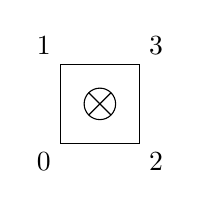
\begin{tikzpicture}
  \draw (0,0) node[below left] {0}
     -- (1,0) node[below right] {2}
     -- (1,1) node[above right] {3}
     -- (0,1) node[above left] {1}
     --cycle;
  \coordinate (c) at (.5,.5);
  \draw (c) circle (.2);
  \draw (c) +(45:.2) -- +(45:-.2)
            +(-45:.2) -- +(-45:-.2);
\end{tikzpicture}
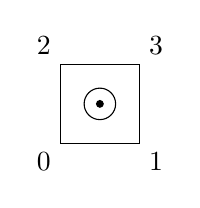
\begin{tikzpicture}
  \draw (0,0) node[below left] {0}
     -- (1,0) node[below right] {1}
     -- (1,1) node[above right] {3}
     -- (0,1) node[above left] {2}
     --cycle;
  \coordinate (c) at (.5,.5);
  \draw (c) circle (.2);
  \fill (c) circle (.05);
\end{tikzpicture}

Note that if you omit the index/id with the value 3 both the cyclic and the
acyclic case reduce to the triangle case.

\subsection{Case studies for particular finite element families}

\subsubsection{P1}

\section{Appendix: List of Available Elements}



% bibtex bibliography
%\bibliographystyle{plain}
%\bibliography{istl.bib}


\end{document}
